\chapter{Программная реализация}

Экспериментальным путем было решено разбить решение задачи детекции активаций
на две части. Первая часть --- поиск области активации с помощью
сегментирующей нейронной сети, вторая --- поиск прямыми методами точки
интереса.

Для реализации использовался язык программирования Python, а так же такие библиотеки как:

\begin{itemize}
	\item PyTorch: построение модели, обучение и предсказание
	\item NumPy: чтение/запись и предобработка записей сигналов и разметки
	\item SciPy: предобработка записей сигналов
	\item mlflow: хранение информации об экспериментах и отслеживание метрик
	\item ONNX: предсказание
	\item DearPyGui: графический интерфейс для некоторых вспомогательных программ
\end{itemize}

\noindent Исходный код с реализацией функционала описанного в этой главе содержится
в \cite{heartbeat-detector-source,egm-analyzer-source}.

\section{Модель}

В качестве нейронной сети для сегментации сигнала была выбрана модель типа
"UNet". Выбор пал на нее, так как уже были работы, где она себя хорошо
зарекомендовала в схожей задаче \cite{victor}. В целом, это достаточно похожая
на оригинал одномерная версия модели. Однако не обошлось и без модификаций:

\begin{enumerate}

	\item Паддинг: для сохранения размера вектора при свертках используется
	паддинг с зеркальным заполнением. Так же это позволяет получить равный по
	размеру входу выход.

	\item Upsample: вместо обратных сверток на этапе восстановления
	используется upsample. Это необучаемая часть нейросети, поэтому обучение и
	предсказание занимает заметно меньше времени.

\end{enumerate}

Сама модель состоит только из сверток, pooling слоев и слоев upsample, то есть
не включает в себя полносвязные слои. Можно выделить две части: ``спуск'' и
``подъем''. Каждый слой спуска состоит из двух последовательных сверток и слоя
max pool. Слой же подъема почти в точности повторяет спуск с тем отличием, что
выполняет обратную операцию, в связи с чем вместо max pool использует upsample.
Так же в архитектуре присутствуют остаточные связи, они соединяют
соответствующие части спуска и подъема посредством конкатенации тензоров. Важно
отметить, что перед всеми слоями max pooling используются слои dropout для
борьбы с переобучением и повышения обобщающей способности модели
\cite{cnn-dropout}. Наглядно нейросеть изображена на рис. \ref{fig:unet}.

\begin{figure}[!htb]
	\centering
	\includegraphics[width=\textwidth]{unet.png}
	\caption{Архитектура нейронной сети UNet}
	\label{fig:unet}
\end{figure}

Так как записи сигналов могут иметь разное количество каналов, было решено, что
нейросеть будет сегментировать по одному каналу за раз вместо нескольких или
даже всех. Далее исходя из компромисса между доступными ресурсами и желанием
подавать на вход нейросети как можно больший сигнал, было решено остановится на
размере входа в 10000 сэмплов, что в нашем случае (при дискретизации в 5 кГц)
эквивалентно 2 секундам. Полный описание модели приведено в приложении (см.
\hyperref[lst:unet]{Описание нейронной сети})

\subsection{Обучение}

Обучение нейронной сети производилось на компьютере со следующими характеристиками:

\begin{enumerate}
	\item GPU: Nvidia GeForce RTX3070 (8Гб видеопамяти)
	\item RAM: 32Гб
	\item CPU: Intel Core i5 12400 (6 ядер x 2.5 Ггц)
\end{enumerate}

В качестве метода оптимизации использовался adam (как один из самых продвинутых
методов стохастического градиентного спуска \cite{adam}) в паре с milestone
планировщиком для динамического контроля learning rate во время обучения.

В качестве функции потерь в данной работе использована комбинация (сумма) бинарной
кросс-энтропии и функции потерь Dice. Такой выбор обусловлен стремлением к
достижению оптимального баланса между двумя аспектами: точностью сегментации
сигнала и стабильностью обучения модели. Функция потерь Dice хорошо подходит
для задач сегментации, однако, может быть нестабильной в определенных ситуациях
из-за своей невыпуклой природы. Для сохранения относительной стабильности
обучения и предотвращения возможных проблем с градиентным спуском, была введена
инарная кросс-энтропия.

Как было упомянуто ранее, набор данных несбалансирован, что делает некоторые
метрики, например, точность (accuracy), неподходящими для оценки качества
предсказаний. Однако, в таких случаях хорошо подходит F-мера, которая
учитывает как полноту, так и точность предсказаний, именно поэтому она была
выбрана для данной задачи.

\subsubsection{Отслеживание экспериментов и метрик}

Благодаря тому, что в стеке используемых технологий есть язык программирования
Python, открывается возможность использования разнообразных библиотек для
удобства отслеживания экспериментов. В данном случае была выбрана библиотека
mlflow. Использовалась она для хранения информации о параметрах экспериментов,
таких как, например, learning rate, test fold, файл с реализаций нейронной
сети, loss, а так же для отслеживания метрик моделей (см. рис.
\ref{fig:mlflow-metrics}). В качестве такой метрики была loss функция. Она
записывалась на каждом пакете и эпохе.

\begin{figure}[!htb]
	\centering
	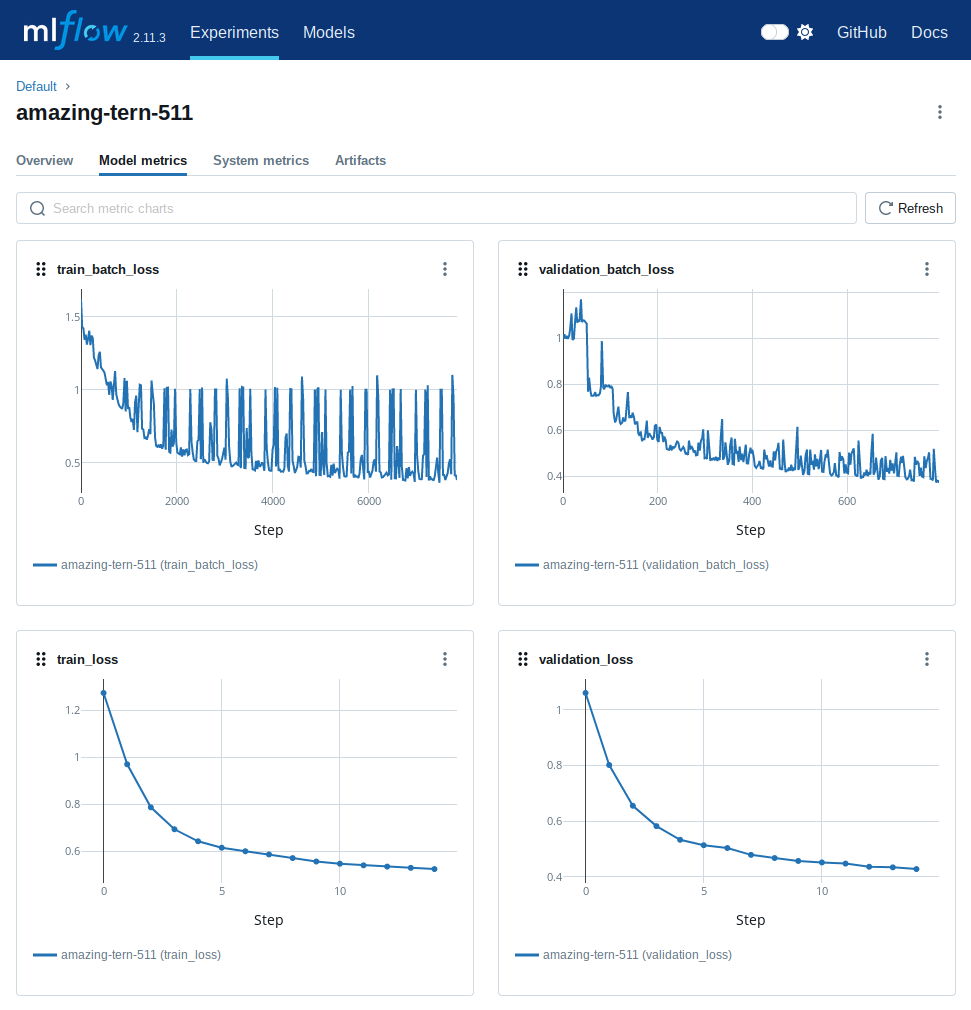
\includegraphics[width=\textwidth]{mlflow-metrics.png}
	\caption{Пример отображения метрик для эксперимента в mlflow}
	\label{fig:mlflow-metrics}
\end{figure}

\subsection{Предсказание}
\subsubsection{Предобработка}

При предсказании необходимо привести вход к виду, максимально приближенному к
тому, какой имели записи сигналов, на которых обучалась нейросеть. В связи с
чем в предсказании появляется шаг предобработки, полностью повторяющий
процедуры, которые использовались для генерации датасета, а именно: децимацию,
фильтрацию и масштабирование.

\subsubsection{Применение нейронной сети}

На вход программе может подаваться сигнал произвольной длины с любым
количеством каналов. Из-за этого предсказание построено путем обработки одного
канала за раз. Так же важно отметить, что из-за особенностей архитектуры UNet
на концах предсказания могут появляться нежелательные артефакты. Ввиду этого
вместо обычной последовательной итерации по сигналу (сначала обрабатываем часть
сигнала, равного длине входа, далее следующую и так далее) используется
итерация с пересечением и отбрасыванием частей предсказания с начала и конца. В
экспериментах в качестве предсказания бралось 80\% исходного предсказания (то
есть отбрасывалось 10\% с начала предсказания и 10\% --- с конца).

\section{Постобработка}
Сырой выход модели представляет собой тензор таких же размеров, что и вход,
который содержит вероятности наличия активации в каждой точке входного сигнала.
Однако, для нас интересны конкретные активации. Поэтому после предсказания
моделью строятся отрезки поиска активаций. Эти отрезки представляют собой
последовательные участки сигнала с вероятностями нахождения в них активаций
больше заданного порога.

Активация в данной работе определяется как точка максимального спада сигнала,
то есть, формально говоря, это минимум первой производной от кривой сигнала.
Для поиска этой точки на искомых участках предлагается строить сплайн и
рассчитывать его производную для более точного определения искомой точки
активации. Найденные таким образом точки считаются конечным результатом работы
программы.

\section{Анализ ошибок}

Важную роль в процессе улучшения программы играет анализ ошибок, именно
благодаря ему был улучшен изначальный алгоритм, который по точности был сравним
с исходной разметкой. Для этой возможности была разработана специальная
программа с графическим пользовательским интерфейсом (см. рис.
\ref{fig:error-analyser}). Программа позволяет:

\begin{enumerate}

	\item Просматривать случайные ошибки: С помощью программы можно
	просматривать случайные ошибки, которые допустила модель при обнаружении
	активаций в сигналах ЭГ. Это помогает исследователям лучше понять причины
	ошибок и выявить особенности сигналов, которые могут привести к
	неправильному обнаружению. Ошибка выбирается случайно, так как их общее
	количество может варьироваться от нескольких сотен до тысяч, что не дает
	возможности исследователю ознакомится с ними всеми.

	\item Отображать промежуток активации нейросети: Программа помечает
	промежуток сигнала, в котором модель обнаружила активацию выше заданного
	порога. Это позволяет анализировать, насколько корректно модель определяет
	временные интервалы активности.

	\item Показывать оригинальную разметку: Для сравнения результатов модели с
	истинной разметкой сигналов ЭГ программа отображает оригинальную разметку
	данных, что помогает выявлять различия между предсказаниями модели и
	истинной разметкой.

	\item Определять тип ошибки: Программа классифицирует ошибки модели и
	указывает их тип. Например, это может быть ложное срабатывание (false
	positive), когда модель ошибочно обнаруживает активацию там, где ее нет,
	или пропуск активации (false negative), когда модель не обнаруживает
	наличие активации.

	\item Просматривать смежные каналы: Для более полноценного анализа сигналов
	ЭГ программа позволяет просматривать смежные каналы для учета
	исследователями контекста и особенностей сигнала на других каналах при
	анализе ошибок.

\end{enumerate}


\begin{figure}[!htb]
	\centering
	\label{fig:error-analyser}
	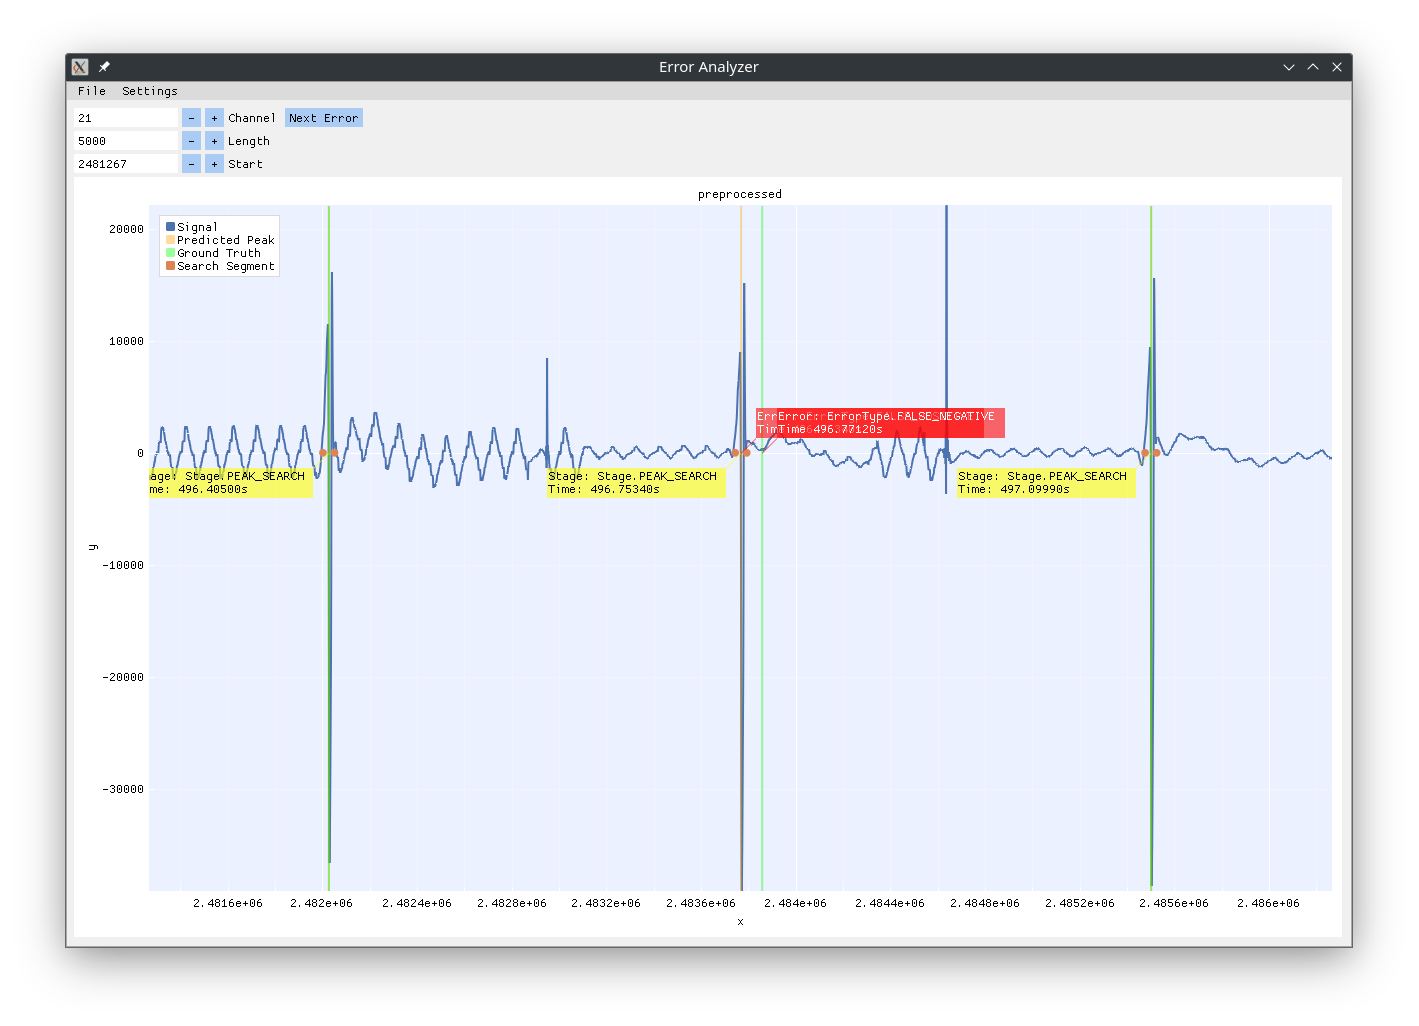
\includegraphics[width=\textwidth]{error-analyzer.png}
	\caption{Пользовательский интерфейс программы для анализа ошибок предсказания}
\end{figure}

\section{Подсчет метрик}

После получения предсказания встает вопрос о подсчете метрик, ведь при прямом
сравнении, метки с предсказания и с разметки могут быть смещены относительно
друг друга, например, на несколько сэмплов. С учетом пожеланий предметного
специалиста, для исследований которого предоставлялось разметка, было решено
считать истинно положительной активацию, которая была предсказана с точностью
до 5 сэмплов. Таким образом алгоритм подсчета выглядел следующим образом:

Для подсчета TP и FP производилась итерация по активациям предсказания. В
окрестности в 5 сэмплов от каждой метки производился поиск наличия таковой в
исходной разметке. В случае положительного результата предсказание считалось
как TP, иначе --- FP. Для подсчета FN итерация происходила по активациям исходной
разметке, а поиск --- по предсказанию. Активация считалась FN в случае
отсутствия результатов поиска в окрестности истинной метки. Наглядно это
изображено на рис. \ref{fig:metrics} (желтым выделен сигнал, по меткам которого
происходит итерация).

\begin{figure}[!htb]
	\centering
	\label{fig:metrics}
	\subfigure[]{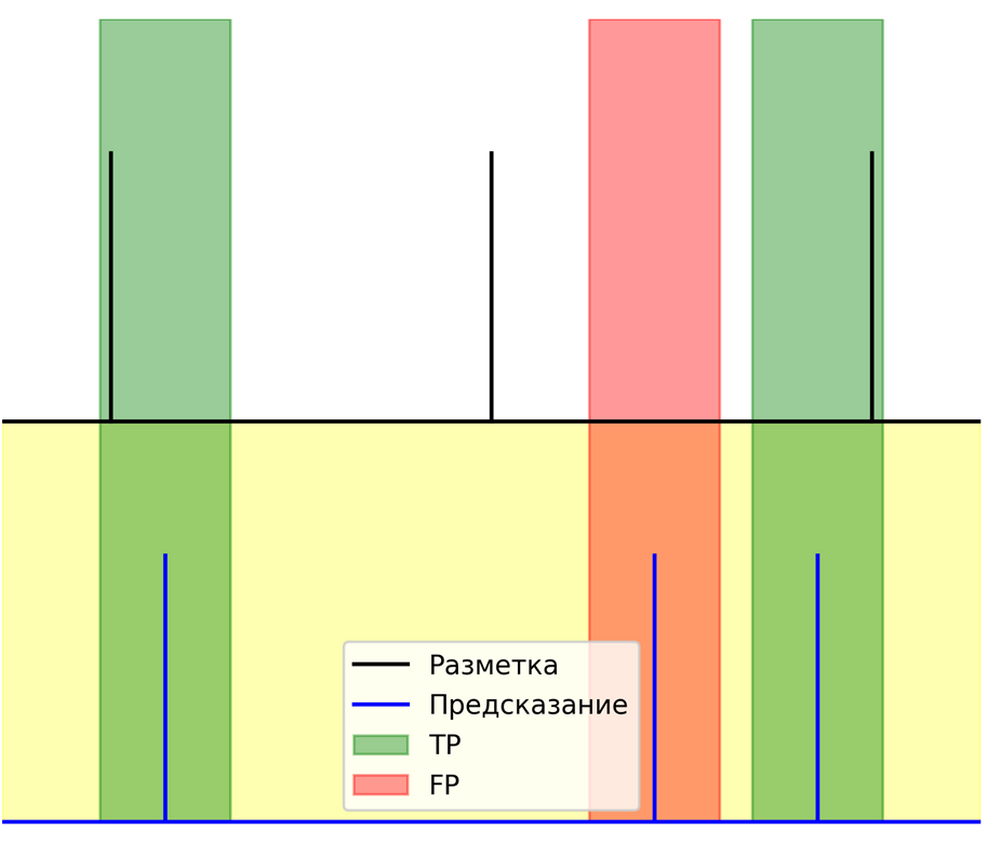
\includegraphics[width=.49\textwidth]{metrics1.png}}
	\subfigure[]{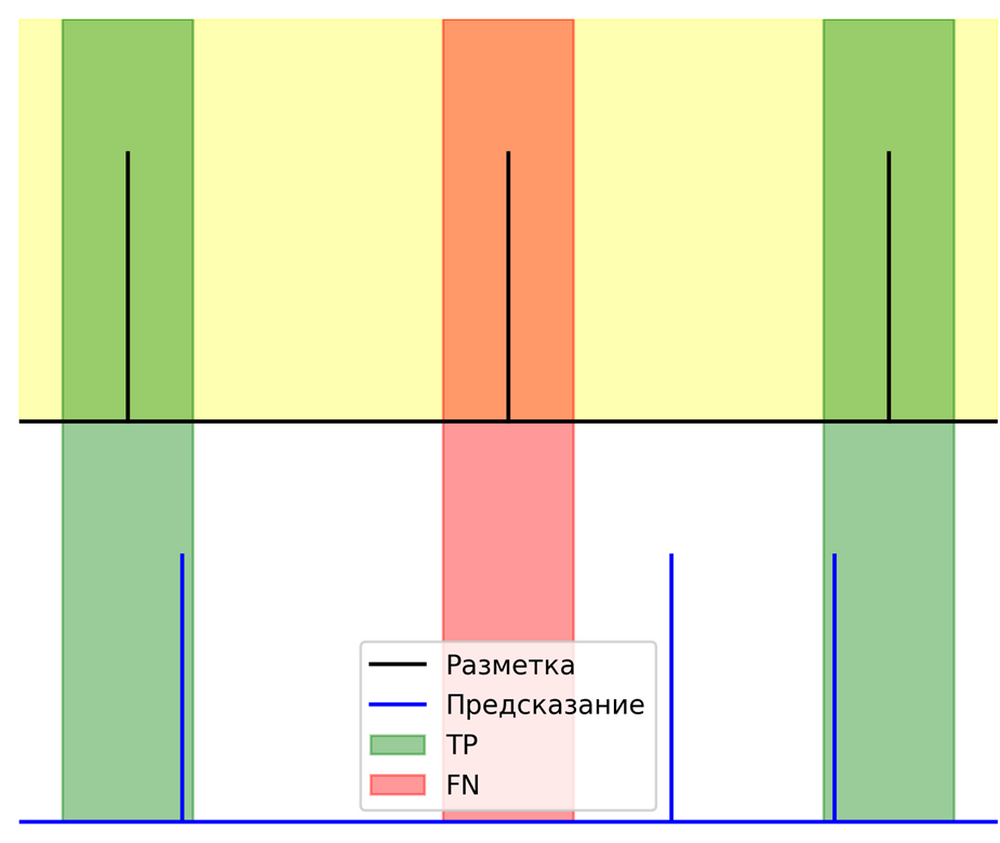
\includegraphics[width=.49\textwidth]{metrics2.png}}
	\caption{(a) Подсчет TP и FP (b) Подсчет FN}
\end{figure}

После подсчета TP, FP и FN по формулам, описанным выше, вычисляется F1-score.
